\documentclass[11pt]{article}
\usepackage[a4paper,margin=1in]{geometry}
\usepackage[T1]{fontenc}
\usepackage{microtype}
\usepackage{amsmath,amssymb,amsthm,mathtools}
\usepackage{enumitem}
\usepackage{booktabs}
\usepackage{tikz}
\usetikzlibrary{arrows.meta}
\PassOptionsToPackage{hyphens}{url}
\usepackage[hidelinks]{hyperref}

\setlength{\parskip}{0.45em}
\setlength{\parindent}{0pt}

% ---------------------------------------------------------------- theorem styles
\theoremstyle{plain}
\newtheorem{theorem}{Theorem}[section]
\newtheorem{lemma}[theorem]{Lemma}
\newtheorem{proposition}[theorem]{Proposition}
\newtheorem{corollary}[theorem]{Corollary}
\newtheorem{citedtheorem}[theorem]{Cited Theorem}
\newtheorem{maintheorem}{Theorem}
\renewcommand{\themaintheorem}{\Alph{maintheorem}}
\newtheorem{maincorollary}[maintheorem]{Corollary}
\newtheorem{mainproposition}[maintheorem]{Proposition}
\theoremstyle{definition}
\newtheorem{definition}[theorem]{Definition}
\newtheorem{hypothesis}[theorem]{Standing Hypothesis}
\newtheorem{example}[theorem]{Example}
\newtheorem{question}[theorem]{Question}
\theoremstyle{remark}
\newtheorem{remark}[theorem]{Remark}

% ---------------------------------------------------------------- notation
\newcommand{\LG}{L(G)}
\newcommand{\st}[1]{E(#1)}
\newcommand{\dout}{d^{+}}
\newcommand{\din}{d^{-}}
\newcommand{\chil}{\operatorname{ch}'}
\newcommand{\chie}{\chi'}
\newcommand{\half}{\tfrac{k-1}{2}}
\newcommand{\why}[1]{\unskip\ \textit{[#1]}}
\newenvironment{steps}{\begin{enumerate}[label=(\arabic*),leftmargin=2.2em,itemsep=0.35em]}{\end{enumerate}}

\title{For Regular Graphs, Galvin's Kernel Method\\Works Only on Bipartite Graphs}
\author{Siddharth Narayan Mishra}
\date{12 October 2026}

\begin{document}
\maketitle

\begin{abstract}
Galvin proved the List Edge Colouring Conjecture for bipartite graphs. His proof gives, for
every bipartite graph $G$ of maximum degree $\Delta$, an orientation of the line graph $\LG$ in
which every induced subgraph has a kernel and every vertex has out-degree at most $\Delta-1$.
The kernel lemma of Bondy, Boppana and Siegel then turns this orientation into a list edge
colouring of $G$ from any lists of size $\Delta$. We prove the reverse direction for regular
graphs: if $G$ is a simple $k$-regular graph and $\LG$ has such an orientation with every
out-degree at most $k-1$, then $G$ is bipartite. With Galvin's theorem this is a
characterisation. We also prove that on a simple regular bipartite graph every such orientation
is one of Galvin's own orientations. So, on simple regular graphs, the kernel method with lists
of size $\Delta$ is exactly Galvin's theorem and nothing more, and it cannot prove the List
Edge Colouring Conjecture for any non-bipartite regular graph. The proof is elementary. It is
written in very small steps, and every fact it uses is proved here from the definitions, so
that it can be checked line by line.
\end{abstract}

\tableofcontents
\newpage

%=================================================================================================
\section{How to read this document}
%=================================================================================================

\paragraph{Purpose.} This document exists so that the proof of Theorem~\ref{thm:main} can be
checked for correctness. Every step is written out, and every step says, in square brackets
and italics, which earlier definition or lemma justifies it. A reader who checks each bracket
has checked the proof.

\paragraph{What is proved and what is cited.} Two results of other authors are stated and
\emph{not} proved here: Galvin's theorem (Cited Theorem~\ref{thm:galvin}) and the kernel lemma
(Cited Theorem~\ref{thm:kernel-lemma}). They are labelled ``Cited Theorem''. They explain why
the main theorem matters and give the ``if'' half of Corollary~\ref{cor:char}, but \textbf{the
proof of the main theorem uses neither of them}. Everything the main proof uses is proved in
Sections~\ref{sec:numbers} to~\ref{sec:digraphs}, from the definitions. Section~\ref{sec:impact}
also describes results of other papers; those descriptions are cited, not proved.

\paragraph{Layout.}
\begin{itemize}[itemsep=0.2em]
  \item Section~\ref{sec:results} states the problem and the results, says what the main
    theorem does not claim, and explains why it is not automatic.
  \item Sections~\ref{sec:numbers}, \ref{sec:graphs} and~\ref{sec:digraphs} prove every
    background fact the proof needs: small facts about numbers, graphs and directed graphs.
  \item Section~\ref{sec:setting} fixes the hypothesis of the main proof.
  \item Sections~\ref{sec:step1} to~\ref{sec:step8} are the proof, in eight steps.
    Section~\ref{sec:proof-main} puts the steps together.
  \item Section~\ref{sec:examples} runs the proof on small graphs.
  \item Sections~\ref{sec:rigidity} and~\ref{sec:twoway} prove two extensions: rigidity, and
    orientations with arcs in both directions.
  \item Section~\ref{sec:impact} explains the impact of the result.
    Section~\ref{sec:computation} reports an independent computer check, and
    Section~\ref{sec:novelty} reports what was checked in the literature.
\end{itemize}

\paragraph{Conventions.} All graphs and digraphs are finite. $\mathbb{Z}$ is the set of
integers. For an integer $\ell\ge 1$, ``indices modulo $\ell$'' means that $a_{\ell+1}$ is
$a_1$, $a_0$ is $a_\ell$, and so on. ``Iff'' means ``if and only if''. The symbol $\equiv$
means congruence modulo $2$ unless stated otherwise. A set with one element is written
$\{x\}$, and $|S|$ is the number of elements of a set $S$.

\paragraph{Relation to the earlier write-up.} The repository note
\path{lecc-small/03-regular-bipartite-theorem.md} proves the same theorem in nine steps.
Steps~1 to~3 here are the same as there. From Step~4 on, this document follows a shorter route:
the orientation $O$ of Section~\ref{sec:step4} also orients the edges of middle rank, in both
directions, so it is balanced for every $k$, and a single parity argument
(Sections~\ref{sec:step6} to~\ref{sec:step8}) replaces the separate treatment of $k$ even and
$k$ odd in Steps~7 to~9 of the note. The two proofs prove the same statement.

%=================================================================================================
\section{The problem and the results}\label{sec:results}
%=================================================================================================

\subsection{List edge colouring}

Let $G$ be a graph with vertex set $V$ and edge set $E$ (the precise definitions are in
Section~\ref{sec:graphs}). Two edges are \emph{adjacent} if they share an end.

\begin{definition}[edge colourings]
\begin{enumerate}[label=(\alph*)]
  \item A \emph{proper edge colouring} of $G$ is a map $c$ from $E$ to some set of colours such
    that adjacent edges get different colours. The \emph{chromatic index} $\chie(G)$ is the
    least number of colours in a proper edge colouring.
  \item A \emph{list assignment} gives every edge $e$ a finite set $C(e)$ of colours, its
    \emph{list}. A proper edge colouring $c$ \emph{respects} the lists if $c(e)\in C(e)$ for
    every edge $e$.
  \item The \emph{list chromatic index} $\chil(G)$ is the least integer $t$ such that for
    \emph{every} list assignment with $|C(e)|\ge t$ for all $e$ there is a proper edge colouring
    respecting the lists.
\end{enumerate}
\end{definition}

If all lists are equal to the same set of $t$ colours, a colouring respecting the lists is just
a proper edge colouring with $t$ colours. So $\chie(G)\le\chil(G)$ for every graph.

\begin{remark}[context, cited]
Edges at one vertex need different colours, so $\chie(G)\ge\Delta(G)$, the maximum degree.
Vizing's theorem~\cite{vizing} says $\chie(G)\le\Delta(G)+1$ for simple graphs. A graph is of
\emph{class one} if $\chie(G)=\Delta(G)$ and of \emph{class two} if $\chie(G)=\Delta(G)+1$.
König's theorem~\cite{konig} says every bipartite graph is of class one. Nothing in the proof
of the main theorem uses these facts.
\end{remark}

\begin{quote}
\textbf{List Edge Colouring Conjecture (LECC).} For every graph $G$, $\chil(G)=\chie(G)$.
\end{quote}

The conjecture is open. It is known for bipartite graphs (Galvin~\cite{galvin}), for $d$-regular
$d$-edge-colourable planar graphs (Ellingham and Goddyn~\cite{eg}), for complete graphs $K_{p+1}$
with $p$ an odd prime (Schauz~\cite{schauz14}), and for several other families.

\subsection{Kernels and the kernel lemma}

The definitions of digraph, orientation, induced subdigraph and out-degree are in
Section~\ref{sec:digraphs}.

\begin{definition}[kernel]\label{def:kernel-intro}
Let $D$ be a digraph with vertex set $X$. A \emph{kernel} of $D$ is a set $K\subseteq X$ such
that
\begin{enumerate}[label=(K\arabic*)]
  \item \emph{(independent)} no arc of $D$ has both ends in $K$, and
  \item \emph{(absorbing)} every vertex $x\in X\setminus K$ has an out-neighbour in $K$, that is,
    there is $y\in K$ with an arc $x\to y$.
\end{enumerate}
$D$ is \emph{kernel-perfect} if for every nonempty $S\subseteq X$ the induced subdigraph $D[S]$
has a kernel.
\end{definition}

This is the definition used in Proofs from THE BOOK~\cite[Chapter~33, Definition~1]{book}.

\begin{citedtheorem}[kernel lemma; Bondy, Boppana and Siegel; see {\cite[Chapter~33, Lemma~1]{book}}]\label{thm:kernel-lemma}
Let $D$ be a kernel-perfect digraph with vertex set $X$, and let every $x\in X$ have a list
$C(x)$ with $|C(x)|\ge \dout(x)+1$. Then the vertices can be coloured from their lists so that
the two ends of every arc get different colours.
\end{citedtheorem}

A proper edge colouring of $G$ is the same thing as a proper vertex colouring of the line graph
$\LG$ (Definition~\ref{def:line-graph}): the vertices of $\LG$ are the edges of $G$, adjacent
when they share an end. This gives the method.

\begin{definition}[certificate]\label{def:certificate}
Let $G$ be a graph and $k\ge 1$ an integer. A \emph{$k$-certificate} for $G$ is an orientation
$D$ of $\LG$ such that
\begin{enumerate}[label=(C\arabic*)]
  \item $D$ is kernel-perfect, and
  \item $\dout_D(e)\le k-1$ for every edge $e$ of $G$.
\end{enumerate}
\end{definition}

By Cited Theorem~\ref{thm:kernel-lemma}, applied to $D$ with lists of size $k\ge\dout(e)+1$, a
$k$-certificate proves $\chil(G)\le k$. When $k=\chie(G)$ this proves the LECC for $G$. We call
this route \emph{the kernel method with lists of size $k$}. It is the method of
Galvin~\cite{galvin}.

\subsection{Galvin's theorem: the forward direction}

\begin{citedtheorem}[Galvin~\cite{galvin}]\label{thm:galvin}
Let $G$ be a bipartite multigraph with maximum degree $\Delta$. Then $\LG$ has a kernel-perfect
orientation with every out-degree at most $\Delta-1$. In particular $G$ has a
$\Delta$-certificate, and $\chil(G)=\chie(G)=\Delta$.
\end{citedtheorem}

The orientation is built from a proper edge colouring $c$ with colours $0,1,\dots,\Delta-1$ and
a bipartition $(A,B)$: at a vertex of $A$ every edge points to the edges of smaller colour, and
at a vertex of $B$ to the edges of larger colour (Definition~\ref{def:galvin-orientation}).
Kernel-perfectness comes from the Gale and Shapley stable matching theorem. An exposition for
the $n\times n$ array is~\cite[Chapter~33]{book}; the same argument works for every bipartite
graph. We do not reprove Galvin's theorem.

\subsection{The results of this document}

\begin{maintheorem}[the reverse direction]\label{thm:main}
Let $k\ge 1$ and let $G$ be a simple $k$-regular graph. If $G$ has a $k$-certificate, then $G$
is bipartite.
\end{maintheorem}

\begin{maincorollary}[characterisation]\label{cor:char}
Let $k\ge 1$ and let $G$ be a simple $k$-regular graph. Then $\LG$ has a kernel-perfect
orientation with every out-degree at most $k-1$ if and only if $G$ is bipartite.
\end{maincorollary}

``If'' is Galvin's theorem; ``only if'' is Theorem~\ref{thm:main}. The proof is in
Section~\ref{sec:proof-main}.

\begin{maintheorem}[rigidity]\label{thm:rigid-intro}
Let $G$ be a simple $k$-regular bipartite graph. Every $k$-certificate for $G$ is a Galvin
orientation $D_c$ for exactly one proper edge colouring $c$ with colours $0,\dots,k-1$.
\end{maintheorem}

This is Theorem~\ref{thm:rigid} in Section~\ref{sec:rigidity}.

\begin{mainproposition}[arcs in both directions]\label{prop:twoway-intro}
Theorem~\ref{thm:main} stays true if the certificate is allowed to join adjacent edges by arcs in
both directions.
\end{mainproposition}

This is Proposition~\ref{prop:twoway} in Section~\ref{sec:twoway}.

\subsection{What the main theorem does not say}\label{sec:not-say}

Theorem~\ref{thm:main} is about the \emph{method}, not about the \emph{number} $\chil(G)$.

\begin{itemize}
  \item It does \textbf{not} say that $\chil(G)>\Delta$ for non-bipartite regular $G$. That
    stronger statement is false. $K_4$ is $3$-regular and contains a triangle, so it is not
    bipartite, yet $\chil(K_4)=3$: this is Schauz's theorem for $K_{p+1}$ with
    $p=3$~\cite{schauz14}, and also the theorem of Ellingham and Goddyn, since $K_4$ is planar and
    has a proper edge colouring with $3$ colours~\cite{eg}. Theorem~\ref{thm:main} says only that
    no $3$-certificate for $K_4$ exists, so the kernel method cannot be the proof of
    $\chil(K_4)=3$.
  \item It says nothing new about graphs of class two. If $\chie(G)=k+1$, then
    $\chil(G)\ge\chie(G)=k+1>k$, so no proof of $\chil(G)=k$ exists by any method. The theorem
    matters for non-bipartite regular graphs of \emph{class one}, where the LECC predicts
    $\chil(G)=k$.
  \item It is about lists of size exactly $\Delta=k$. With lists of size $k+1$ the kernel method
    does succeed on some non-bipartite regular graphs (Section~\ref{sec:computation}: $K_4$ and
    the triangular prism).
  \item It is about simple graphs. The multigraph case is open (Remark~\ref{rem:simple}).
\end{itemize}

\subsection{Why the reverse direction is not automatic}\label{sec:not-automatic}

Galvin's construction needs a bipartition: it points edges one way at vertices of $A$ and the
other way at vertices of $B$. So one might think the reverse direction is obvious, ``Galvin's
method needs bipartite graphs''. It is not obvious, for three reasons.

\begin{enumerate}[label=(\roman*)]
  \item The kernel lemma (Cited Theorem~\ref{thm:kernel-lemma}) works on \emph{every} digraph.
    Galvin's recipe is one way to build a certificate. It does not show that no other recipe
    exists. A non-bipartite graph could, a priori, have a certificate built some other way.
  \item Certificates on non-bipartite graphs do exist once a hypothesis is dropped. The diamond
    ($K_4$ minus an edge) is not bipartite, has maximum degree $3$, and has $3$-certificates
    (Example~\ref{ex:diamond}); it is not regular. $K_4$ is regular and not bipartite, and has
    $4$-certificates (Section~\ref{sec:computation}); there the lists have size $\Delta+1$.
    McDonald~\cite{mcd} gives further examples of both kinds: every ``bipartite plus an edge''
    graph~\cite[Theorem~3]{mcd}, and the Petersen graph with lists of size
    $4=\Delta+1$~\cite[Theorem~4]{mcd}.
  \item The known negative results are weaker. McDonald~\cite[Theorem~5]{mcd} shows that $K_n$
    ($n\ge 4$) has no certificate of Galvin's special form; Theorem~\ref{thm:main} excludes \emph{every}
    orientation, for \emph{every} non-bipartite regular graph.
\end{enumerate}

So the question ``can some orientation, not Galvin's, prove $\chil(G)=\Delta$ for a
non-bipartite regular graph by the kernel lemma?'' was open as far as we could find, and
Theorem~\ref{thm:main} answers it: no. Theorem~\ref{thm:rigid-intro} adds that on regular
bipartite graphs there is no orientation beyond Galvin's either.

\subsection{The proof in one paragraph, and the roadmap}\label{sec:roadmap}

Take a $k$-certificate $D$. At each vertex $u$ the $k$ edges at $u$ are pairwise adjacent in
$\LG$, so $D$ orders them; this gives each edge a \emph{rank} $0,1,\dots,k-1$ at each of its two
ends (Step~1). Counting arcs shows every out-degree is exactly $k-1$, which forces the two ranks
of every edge to add up to $k-1$ (Step~2). An odd cycle of $G$ along which every vertex ranks
its next edge better than its previous edge would become a directed odd cycle in $D$, which has
no kernel; so there is no such ``odd ring'' (Step~3). Now orient $G$ itself: $u\to v$ when $u$
ranks $uv$ in the better half (Step~4). Every directed cycle of length at least $3$ of this
orientation is a ring (Step~5), so it has no directed cycle of odd length and no directed closed
walk of odd length (Step~6). Each vertex has as many out-arcs as in-arcs, so every arc can be
walked back, and the way back always has odd length (Step~7). Then every cycle of $G$ can be
turned into a directed closed walk of the same parity, which must be even (Step~8). A graph with
no odd cycle is bipartite.

\begin{center}
\small
\begin{tabular}{@{}lll@{}}
\toprule
Step & Statement & Uses \\
\midrule
1 & ranks exist; $\dout(uv)=r_u(v)+r_v(u)$ & Lemmas~\ref{lem:tournament}, \ref{lem:line-graph}, \ref{lem:hereditary} \\
2 & $r_u(v)+r_v(u)=k-1$ & Step 1, Lemmas~\ref{lem:sum-outdeg}, \ref{lem:line-graph} \\
3 & no odd ring & Step 1, Lemmas~\ref{lem:cycle-edges}, \ref{lem:odd-dicycle} \\
4 & the orientation $O$ of $G$ is balanced & Step 2, Lemma~\ref{lem:halves} \\
5 & directed cycles of $O$ of length $\ge 3$ are rings & Steps 1, 2, 4 \\
6 & $O$ has no odd directed closed walk & Steps 3, 5, Lemma~\ref{lem:odd-diwalk} \\
7 & every arc of $O$ can be walked back, in an odd number of steps & Steps 4, 6, Lemma~\ref{lem:balanced} \\
8 & every cycle of $G$ is even & Steps 4, 7, Lemma~\ref{lem:parity} \\
end & $G$ is bipartite & Step 8, Lemma~\ref{lem:bipartite} \\
\bottomrule
\end{tabular}
\end{center}

%=================================================================================================
\section{Preliminaries on numbers}\label{sec:numbers}
%=================================================================================================

\begin{lemma}[pairs]\label{lem:pairs}
A set with $t$ elements has exactly $t(t-1)/2$ subsets with two elements.
\end{lemma}

\begin{proof}
\begin{steps}
  \item The number of ordered pairs $(x,y)$ of distinct elements is $t(t-1)$: there are $t$
    choices for $x$ and then $t-1$ choices for $y\ne x$.
  \item Each two-element subset $\{x,y\}$ arises from exactly two ordered pairs, $(x,y)$ and
    $(y,x)$.
  \item So the number of two-element subsets is $t(t-1)/2$. \qedhere
\end{steps}
\end{proof}

\begin{lemma}[upper and lower halves]\label{lem:halves}
Let $k\ge 1$ and let $R=\{0,1,\dots,k-1\}$. Put
\[
  R_{\le}=\{r\in R : r\le \half\},\qquad R_{\ge}=\{r\in R : r\ge \half\}.
\]
Then $|R_{\le}|=|R_{\ge}|$.
\end{lemma}

\begin{proof}
\begin{steps}
  \item Define $\phi(r)=k-1-r$. If $0\le r\le k-1$ then $0\le k-1-r\le k-1$. So $\phi$ maps $R$
    to $R$.
  \item $\phi(\phi(r))=k-1-(k-1-r)=r$. So $\phi$ is its own inverse, hence a bijection of $R$.
  \item For $r\in R$: $r\le\half$ iff $-r\ge-\half$ iff $k-1-r\ge k-1-\half=\half$. So
    $r\in R_{\le}$ iff $\phi(r)\in R_{\ge}$.
  \item By (2) and (3), $\phi$ restricts to a bijection from $R_{\le}$ to $R_{\ge}$. So the two
    sets have the same size. \qedhere
\end{steps}
\end{proof}

\begin{remark}
In fact $|R_{\le}|=|R_{\ge}|=\lceil k/2\rceil$, but only the equality of the two sizes is used.
If $k$ is odd, then $\half$ is an integer and lies in both sets. If $k$ is even, the two sets are
disjoint.
\end{remark}

\begin{lemma}[parity of a sum of odd numbers]\label{lem:parity}
If $q_1,\dots,q_\ell$ are odd integers, then $q_1+\dots+q_\ell\equiv\ell\pmod 2$.
\end{lemma}

\begin{proof}
\begin{steps}
  \item Each $q_i$ is odd, so $q_i=2s_i+1$ for some integer $s_i$.
  \item Then $q_1+\dots+q_\ell=2(s_1+\dots+s_\ell)+\ell$, which differs from $\ell$ by an even
    number. \qedhere
\end{steps}
\end{proof}

%=================================================================================================
\section{Preliminaries on graphs}\label{sec:graphs}
%=================================================================================================

\subsection{Definitions}

\begin{definition}[graph]\label{def:graph}
A \emph{simple graph} $G$ is a pair $(V,E)$ of a finite set $V$ of \emph{vertices} and a set $E$
of two-element subsets of $V$, the \emph{edges}. The edge $\{u,v\}$ is written $uv$ (so $uv=vu$),
and $u,v$ are its \emph{ends}. Because $E$ is a \emph{set} of \emph{two-element} subsets:
\begin{itemize}
  \item there are no loops (an edge has two different ends), and
  \item there are no parallel edges (two vertices are joined by at most one edge).
\end{itemize}
A \emph{multigraph} may have parallel edges; it is not a simple graph.
\end{definition}

\begin{definition}[neighbours, stars, degree, regular]
Let $G=(V,E)$ be simple and $u\in V$.
\begin{itemize}
  \item $v$ is a \emph{neighbour} of $u$ if $uv\in E$. $N(u)$ is the set of neighbours.
  \item The \emph{star} of $u$ is $\st{u}=\{e\in E: u\in e\}$, the set of edges at $u$.
  \item The \emph{degree} of $u$ is $d(u)=|\st{u}|$. The map $v\mapsto uv$ is a bijection from
    $N(u)$ to $\st{u}$, so $d(u)=|N(u)|$ as well.
  \item $G$ is \emph{$k$-regular} if $d(u)=k$ for every $u\in V$. $\Delta(G)$ is the maximum
    degree.
\end{itemize}
\end{definition}

\begin{definition}[walks and cycles]\label{def:walk}
Let $G=(V,E)$ be simple.
\begin{itemize}
  \item A \emph{walk} of \emph{length} $L\ge 0$ from $w_0$ to $w_L$ is a sequence
    $(w_0,w_1,\dots,w_L)$ of vertices with $w_jw_{j+1}\in E$ for $0\le j<L$. Vertices may repeat.
    It is \emph{closed} if $w_L=w_0$.
  \item A \emph{cycle} of \emph{length} $\ell$ is a sequence $(a_1,\dots,a_\ell)$ of
    $\ell\ge 3$ \emph{distinct} vertices such that $a_ia_{i+1}\in E$ for every $i$, indices
    modulo $\ell$. Its \emph{edges} are $e_i=a_ia_{i+1}$ for $i=1,\dots,\ell$. It is \emph{odd}
    or \emph{even} according to $\ell$.
\end{itemize}
\end{definition}

\begin{definition}[bipartite]\label{def:bipartite}
$G=(V,E)$ is \emph{bipartite} if $V$ can be split into two disjoint sets $A$ and $B$
(with $A\cup B=V$) such that every edge has one end in $A$ and one end in $B$. The pair $(A,B)$ is
a \emph{bipartition}.
\end{definition}

\subsection{Basic lemmas}

\begin{lemma}[two edges share at most one end]\label{lem:one-end}
In a simple graph, two distinct edges have at most one common end.
\end{lemma}

\begin{proof}
\begin{steps}
  \item Let $e\ne f$ be edges and suppose they have two common ends $u\ne v$.
  \item $e$ has exactly two elements \why{Definition~\ref{def:graph}} and contains $u$ and $v$,
    so $e=\{u,v\}$. In the same way $f=\{u,v\}$.
  \item So $e=f$, contradicting $e\ne f$. \qedhere
\end{steps}
\end{proof}

This is the only place where the absence of parallel edges enters. Everything later that needs
simplicity goes through this lemma.

\begin{lemma}[handshake]\label{lem:handshake}
For a simple graph, $\sum_{u\in V}d(u)=2|E|$. If $G$ is $k$-regular with $n$ vertices, then
$nk=2|E|$.
\end{lemma}

\begin{proof}
\begin{steps}
  \item Count the pairs $(u,e)$ with $u\in V$, $e\in E$ and $u\in e$.
  \item Grouping by $u$: vertex $u$ is in $|\st{u}|=d(u)$ such pairs. Total $\sum_u d(u)$.
  \item Grouping by $e$: each edge has exactly two ends, so it is in exactly two pairs. Total
    $2|E|$.
  \item The two totals count the same set, so they are equal. If $d(u)=k$ for all $n$ vertices,
    the left side is $nk$. \qedhere
\end{steps}
\end{proof}

\begin{lemma}[edges of a cycle]\label{lem:cycle-edges}
Let $(a_1,\dots,a_\ell)$ be a cycle with edges $e_i=a_ia_{i+1}$ (indices modulo $\ell$). Then:
\begin{enumerate}[label=(\alph*)]
  \item the edges $e_1,\dots,e_\ell$ are pairwise distinct;
  \item for $i\ne j$, the edges $e_i$ and $e_j$ have a common end iff $j\equiv i+1$ or
    $j\equiv i-1\pmod\ell$;
  \item the only common end of $e_{i-1}$ and $e_i$ is $a_i$.
\end{enumerate}
\end{lemma}

\begin{proof}
Throughout, recall that $a_1,\dots,a_\ell$ are distinct and $\ell\ge 3$, so two vertices
$a_p,a_q$ are equal iff $p\equiv q\pmod\ell$.

(a) \begin{steps}
  \item Suppose $e_i=e_j$ with $i\not\equiv j$.
  \item $a_i\in e_i=e_j=\{a_j,a_{j+1}\}$, so $a_i=a_j$ or $a_i=a_{j+1}$. The first means
    $i\equiv j$, which is excluded. So $a_i=a_{j+1}$, that is, $j\equiv i-1$.
  \item $a_{i+1}\in e_j$, so $a_{i+1}=a_j$ or $a_{i+1}=a_{j+1}$. The second means $i\equiv j$,
    which is excluded. So $a_{i+1}=a_j$, that is, $j\equiv i+1$.
  \item By (2) and (3), $i-1\equiv i+1\pmod\ell$, so $\ell$ divides $2$. This contradicts
    $\ell\ge 3$.
\end{steps}

(b) \begin{steps}
  \item $e_i=\{a_i,a_{i+1}\}$ and $e_j=\{a_j,a_{j+1}\}$. A common end is a vertex in both, so one
    of these holds: $a_i=a_j$, $a_i=a_{j+1}$, $a_{i+1}=a_j$, $a_{i+1}=a_{j+1}$.
  \item These mean, respectively, $i\equiv j$, $i\equiv j+1$, $i+1\equiv j$, $i+1\equiv j+1$
    (modulo $\ell$).
  \item The first and the last say $i\equiv j$, which is excluded. The second says
    $j\equiv i-1$. The third says $j\equiv i+1$.
  \item Conversely, if $j\equiv i+1$ then $a_{i+1}=a_j$ is a common end, and if $j\equiv i-1$
    then $a_i=a_{j+1}$ is a common end.
\end{steps}

(c) \begin{steps}
  \item $a_i$ is in $e_{i-1}=\{a_{i-1},a_i\}$ and in $e_i=\{a_i,a_{i+1}\}$.
  \item By (a), $e_{i-1}\ne e_i$. By Lemma~\ref{lem:one-end} they have at most one common end. So
    $a_i$ is the only one. \qedhere
\end{steps}
\end{proof}

\begin{lemma}[odd closed walks contain odd cycles]\label{lem:odd-walk}
If a simple graph has a closed walk of odd length, then it has an odd cycle.
\end{lemma}

\begin{proof}
By strong induction on the length $L$. Let $W=(w_0,\dots,w_L)$ be a closed walk with $L$ odd,
and assume the lemma for all odd lengths smaller than $L$.
\begin{steps}
  \item $L\ne 1$: a closed walk of length $1$ would need $w_0w_1=w_0w_0\in E$, a loop, and there
    are no loops \why{Definition~\ref{def:graph}}. So $L\ge 3$, as $L$ is odd.
  \item \emph{Case 1: $w_0,\dots,w_{L-1}$ are distinct.} Then $(w_0,\dots,w_{L-1})$ is a
    sequence of $L\ge 3$ distinct vertices, consecutive ones are joined by edges, and so are
    $w_{L-1}$ and $w_L=w_0$. This is a cycle of odd length $L$ \why{Definition~\ref{def:walk}}.
  \item \emph{Case 2: $w_i=w_j$ for some $0\le i<j\le L-1$.} Split $W$ into
    \[ W_1=(w_i,w_{i+1},\dots,w_j),\qquad W_2=(w_0,\dots,w_i,w_{j+1},\dots,w_L). \]
    $W_1$ is a closed walk (it starts at $w_i$ and ends at $w_j=w_i$) of length $j-i$. $W_2$ is
    a walk, because $w_iw_{j+1}=w_jw_{j+1}\in E$, and it is closed, of length $i+(L-j)$.
  \item Both lengths are between $1$ and $L-1$, and they add up to $L$, which is odd. So one of
    them is odd and smaller than $L$.
  \item By the induction hypothesis, that shorter closed walk gives an odd cycle. \qedhere
\end{steps}
\end{proof}

\begin{lemma}[no odd cycle implies bipartite]\label{lem:bipartite}
If a simple graph $G$ has no odd cycle, then $G$ is bipartite.
\end{lemma}

\begin{proof}
\begin{steps}
  \item Call $x$ and $y$ \emph{connected} if there is a walk from $x$ to $y$. This is an
    equivalence relation: $(x)$ is a walk of length $0$; a walk reversed is a walk; two walks
    $x\to y$ and $y\to z$ joined at $y$ give a walk $x\to z$. Its classes are the
    \emph{components}.
  \item In each component choose one vertex, its \emph{root}. For each vertex $x$, let $s(x)$
    be the root of its component and $\delta(x)$ the least length of a walk from $s(x)$ to $x$.
    It exists, since such walks exist.
  \item Put $A=\{x:\delta(x)\text{ even}\}$ and $B=\{x:\delta(x)\text{ odd}\}$. They are
    disjoint and cover $V$.
  \item Let $xy\in E$; we show $x,y$ are not both in $A$ and not both in $B$. Suppose
    $\delta(x)\equiv\delta(y)$. The edge $xy$ is a walk, so $x,y$ are in one component and
    $s(x)=s(y)=s$.
  \item Take a shortest walk $P$ from $s$ to $x$ (length $\delta(x)$) and a shortest walk $Q$
    from $s$ to $y$ (length $\delta(y)$). Follow $P$ from $s$ to $x$, then the edge $xy$, then $Q$
    backwards from $y$ to $s$. This is a closed walk of length $\delta(x)+1+\delta(y)$.
  \item Since $\delta(x)\equiv\delta(y)$, the length is $\equiv 2\delta(x)+1\equiv 1$: it is odd.
  \item By Lemma~\ref{lem:odd-walk}, $G$ has an odd cycle, contradicting the hypothesis. So every
    edge has one end in $A$ and one in $B$, and $(A,B)$ is a bipartition. \qedhere
\end{steps}
\end{proof}

\subsection{The line graph}

\begin{definition}[line graph]\label{def:line-graph}
The \emph{line graph} $\LG$ of a simple graph $G=(V,E)$ has vertex set $E$, and two distinct
edges $e,f\in E$ are adjacent in $\LG$ iff they have a common end in $G$.
\end{definition}

To avoid confusion we keep saying \emph{edge} for an element of $E$, also when it is regarded as
a vertex of $\LG$.

\begin{lemma}[structure of the line graph]\label{lem:line-graph}
Let $G=(V,E)$ be simple.
\begin{enumerate}[label=(\alph*)]
  \item For each $u\in V$, any two distinct edges of $\st{u}$ are adjacent in $\LG$.
  \item If $e,f$ are adjacent in $\LG$, they have exactly one common end. Call it $w(e,f)$.
  \item For an edge $e=uv$, the neighbours of $e$ in $\LG$ are the edges of
    $(\st{u}\setminus\{e\})\cup(\st{v}\setminus\{e\})$, and these two sets are disjoint.
  \item If $G$ is $k$-regular with $n$ vertices, then $\LG$ has exactly $nk(k-1)/2=|E|(k-1)$
    edges.
\end{enumerate}
\end{lemma}

\begin{proof}
(a) Two distinct edges of $\st{u}$ both contain $u$, so they have the common end $u$.

(b) They have at least one common end by Definition~\ref{def:line-graph}, and at most one by
Lemma~\ref{lem:one-end}.

(c) \begin{steps}
  \item An edge $f\ne e$ is a neighbour of $e$ iff $f$ contains $u$ or $v$, that is, iff
    $f\in\st{u}\setminus\{e\}$ or $f\in\st{v}\setminus\{e\}$.
  \item If $f$ were in both sets, $f$ and $e$ would have the two common ends $u,v$, which
    Lemma~\ref{lem:one-end} forbids. So the sets are disjoint.
\end{steps}

(d) \begin{steps}
  \item Send every edge $\{e,f\}$ of $\LG$ to the vertex $w(e,f)$ of $G$. By (b) this is
    well defined.
  \item The edges of $\LG$ sent to a fixed vertex $w$ are exactly the two-element subsets of
    $\st{w}$. Indeed, such an edge $\{e,f\}$ has $e,f\in\st{w}$; conversely, any two distinct
    $e,f\in\st{w}$ are adjacent by (a), with common end $w$, and by (b) $w(e,f)=w$.
  \item $|\st{w}|=k$, so by Lemma~\ref{lem:pairs} there are $k(k-1)/2$ such subsets for each $w$.
  \item Summing over the $n$ vertices gives $nk(k-1)/2$ edges of $\LG$.
  \item By Lemma~\ref{lem:handshake}, $nk=2|E|$, so $nk(k-1)/2=|E|(k-1)$. \qedhere
\end{steps}
\end{proof}

%=================================================================================================
\section{Preliminaries on digraphs and kernels}\label{sec:digraphs}
%=================================================================================================

\subsection{Definitions}

\begin{definition}[digraph]\label{def:digraph}
A \emph{digraph} $D$ is a pair $(X,A)$ of a finite set $X$ and a set $A$ of ordered pairs
$(x,y)$ of \emph{distinct} elements of $X$, the \emph{arcs}. The arc $(x,y)$ is written
$x\to y$. So there are no loops and no two equal arcs, but $x\to y$ and $y\to x$ may both be
arcs.
\begin{itemize}
  \item $y$ is an \emph{out-neighbour} of $x$ if $x\to y$. The \emph{out-degree} $\dout_D(x)$ is
    the number of out-neighbours, and the \emph{in-degree} $\din_D(x)$ the number of $z$ with
    $z\to x$.
  \item $D$ is \emph{balanced} if $\dout_D(x)=\din_D(x)$ for every $x\in X$.
  \item For $S\subseteq X$, the \emph{induced subdigraph} $D[S]$ has vertex set $S$ and as arcs
    all arcs of $D$ with both ends in $S$.
  \item An \emph{orientation} of a graph $H$ with vertex set $X$ is a digraph on $X$ such that
    for every edge $xy$ of $H$ exactly one of $x\to y$, $y\to x$ is an arc, and there are no
    other arcs.
  \item A \emph{tournament} is an orientation of a complete graph: between any two distinct
    vertices there is exactly one arc.
\end{itemize}
\end{definition}

\begin{definition}[directed walks and cycles]\label{def:diwalk}
Let $D=(X,A)$ be a digraph.
\begin{itemize}
  \item A \emph{directed walk} of \emph{length} $L\ge 0$ from $w_0$ to $w_L$ is a sequence
    $(w_0,\dots,w_L)$ with $w_j\to w_{j+1}$ for $0\le j<L$. It is \emph{closed} if $w_L=w_0$.
  \item If $W$ is a directed walk from $x$ to $y$ and $W'$ one from $y$ to $z$, their
    \emph{concatenation} $WW'$ (follow $W$, then $W'$) is a directed walk from $x$ to $z$, and its
    length is the sum of the two lengths.
  \item A \emph{directed cycle} of length $\ell\ge 2$ is a sequence $(x_1,\dots,x_\ell)$ of
    distinct vertices with $x_i\to x_{i+1}$ for every $i$, indices modulo $\ell$.
\end{itemize}
\end{definition}

\subsection{Counting and walking}

\begin{lemma}[out-degrees count arcs]\label{lem:sum-outdeg}
$\sum_{x\in X}\dout_D(x)=|A|$. If $D$ is an orientation of a graph $H$, then $|A|$ is the number
of edges of $H$.
\end{lemma}

\begin{proof}
Every arc $x\to y$ is counted exactly once on the left, in $\dout_D(x)$. If $D$ is an
orientation of $H$, each edge of $H$ gives exactly one arc and every arc comes from an edge.
\end{proof}

\begin{lemma}[odd closed directed walks contain odd directed cycles]\label{lem:odd-diwalk}
If a digraph has a closed directed walk of odd length, then it has a directed cycle of odd
length. Every directed cycle of odd length has length at least $3$.
\end{lemma}

\begin{proof}
The second sentence: a directed cycle has length $\ell\ge 2$ by definition, and an odd
$\ell\ge 2$ is at least $3$.

The first sentence, by strong induction on the length $L$ of a closed directed walk
$W=(w_0,\dots,w_L)$ with $L$ odd.
\begin{steps}
  \item $L\ne 1$: that would need an arc $w_0\to w_0$, and digraphs have no loops
    \why{Definition~\ref{def:digraph}}. So $L\ge 3$.
  \item \emph{Case 1: $w_0,\dots,w_{L-1}$ are distinct.} Then $(w_0,\dots,w_{L-1})$ is a
    directed cycle of odd length $L$ \why{Definition~\ref{def:diwalk}; the last arc is
    $w_{L-1}\to w_L=w_0$}.
  \item \emph{Case 2: $w_i=w_j$ for some $0\le i<j\le L-1$.} Then
    $W_1=(w_i,\dots,w_j)$ is a closed directed walk of length $j-i$, and
    $W_2=(w_0,\dots,w_i,w_{j+1},\dots,w_L)$ is a closed directed walk of length $L-(j-i)$, since
    $w_i\to w_{j+1}$ is the arc $w_j\to w_{j+1}$.
  \item Both lengths lie between $1$ and $L-1$ and add up to the odd number $L$, so one of them
    is odd and shorter than $L$. The induction hypothesis applies to it. \qedhere
\end{steps}
\end{proof}

\begin{lemma}[in a balanced digraph every arc can be walked back]\label{lem:balanced}
Let $D=(X,A)$ be a balanced digraph and $x\to y$ an arc. Then there is a directed walk from $y$
to $x$.
\end{lemma}

\begin{proof}
\begin{steps}
  \item Let $R$ be the set of vertices $z$ such that some directed walk goes from $y$ to $z$.
    Then $y\in R$ (walk of length $0$).
  \item \emph{No arc leaves $R$:} if $z\in R$ and $z\to w$, then $w\in R$, since a walk from $y$
    to $z$ followed by the arc $z\to w$ is a walk from $y$ to $w$.
  \item Let $a$ be the number of arcs with both ends in $R$, and $b$ the number of arcs with
    tail outside $R$ and head in $R$.
  \item $\sum_{z\in R}\dout_D(z)$ counts the arcs with tail in $R$. By (2) all of them have head
    in $R$. So the sum is $a$.
  \item $\sum_{z\in R}\din_D(z)$ counts the arcs with head in $R$. Their tails are in $R$ or not.
    So the sum is $a+b$.
  \item $D$ is balanced, so the sums in (4) and (5) are equal: $a=a+b$, hence $b=0$.
  \item The arc $x\to y$ has head $y\in R$. If $x\notin R$, it would be counted in $b=0$. So
    $x\in R$: there is a directed walk from $y$ to $x$. \qedhere
\end{steps}
\end{proof}

\subsection{Kernels}

Kernels and kernel-perfectness were defined in Definition~\ref{def:kernel-intro}.

\begin{lemma}[kernel-perfectness is inherited]\label{lem:hereditary}
If $D$ is kernel-perfect and $T\subseteq X$, then $D[T]$ is kernel-perfect.
\end{lemma}

\begin{proof}
For nonempty $S\subseteq T$, the digraph $(D[T])[S]$ has vertex set $S$ and the arcs of $D[T]$
with both ends in $S$, which are the arcs of $D$ with both ends in $S$. So $(D[T])[S]=D[S]$,
which has a kernel because $D$ is kernel-perfect.
\end{proof}

\begin{lemma}[an odd directed cycle has no kernel]\label{lem:odd-dicycle}
Let $\ell\ge 3$ be odd and let $F$ be a digraph whose vertices are $\ell$ distinct elements
$s_1,\dots,s_\ell$ and whose arcs are exactly $s_i\to s_{i+1}$ for $i=1,\dots,\ell$ (indices
modulo $\ell$). Then $F$ has no kernel.
\end{lemma}

\begin{proof}
Suppose $K$ is a kernel of $F$. Put $\kappa_i=1$ if $s_i\in K$ and $\kappa_i=0$ otherwise.
\begin{steps}
  \item The only out-neighbour of $s_i$ is $s_{i+1}$ \why{the list of arcs}.
  \item If $s_i\notin K$, then $s_i$ has an out-neighbour in $K$ \why{(K2)}, so $s_{i+1}\in K$
    \why{(1)}.
  \item If $s_i\in K$, then $s_{i+1}\notin K$, since the arc $s_i\to s_{i+1}$ would otherwise
    have both ends in $K$ \why{(K1)}.
  \item By (2) and (3), $\kappa_{i+1}=1-\kappa_i$, so $\kappa_{i+1}\equiv\kappa_i+1$ for every $i$.
  \item Applying (4) $\ell$ times, starting at $i=1$: $\kappa_{1+\ell}\equiv\kappa_1+\ell$.
  \item But $s_{1+\ell}=s_1$ (indices modulo $\ell$), so $\kappa_{1+\ell}=\kappa_1$, and (5)
    gives $\ell\equiv 0$. This contradicts $\ell$ odd. \qedhere
\end{steps}
\end{proof}

In words: going around the cycle, membership in $K$ must alternate, and an odd cycle cannot be
coloured alternately.

\begin{lemma}[kernel-perfect tournaments are linear orders]\label{lem:tournament}
Let $T$ be a tournament with $t\ge 1$ vertices in which every induced subdigraph on a nonempty
vertex set has a kernel. Then the vertices of $T$ can be listed as $x_0,x_1,\dots,x_{t-1}$ so
that, for all $i\ne j$,
\[
  x_i\to x_j \text{ is an arc}\iff i>j .
\]
In particular $\dout_T(x_i)=i$, and the out-degrees of the vertices of $T$ are exactly
$0,1,\dots,t-1$, each once.
\end{lemma}

\begin{proof}
By induction on $t$. For $t=1$ there are no arcs, and $x_0$ is the only vertex. Let $t\ge 2$.
\begin{steps}
  \item $T=T[V(T)]$ has a kernel $K$ \why{hypothesis}.
  \item $|K|\le 1$: two distinct vertices of $K$ are joined by an arc, as $T$ is a tournament,
    which (K1) forbids.
  \item $K\ne\varnothing$: otherwise any vertex (there is one, $t\ge 1$) lies outside $K$ and
    must have an out-neighbour in $K=\varnothing$ \why{(K2)}, which is impossible.
  \item So $K=\{s\}$ for one vertex $s$, and by (K2) every other vertex $x$ has the arc
    $x\to s$. Put $x_0=s$.
  \item Let $T'=T[V(T)\setminus\{s\}]$. It is a tournament with $t-1\ge 1$ vertices, and each of
    its induced subdigraphs is an induced subdigraph of $T$ (as in Lemma~\ref{lem:hereditary}),
    so it has a kernel.
  \item By the induction hypothesis, list the vertices of $T'$ as $x_1,\dots,x_{t-1}$ with
    $x_i\to x_j$ iff $i>j$, for $i,j\ge 1$. Arcs of $T'$ are exactly the arcs of $T$ between
    these vertices, so this holds in $T$.
  \item Pairs involving $x_0$: for $i\ge 1$, $x_i\to x_0$ by (4), which agrees with $i>0$. And
    $x_0\to x_i$ is not an arc, because exactly one of the two arcs is present; this agrees with
    $0>i$ being false.
  \item The out-neighbours of $x_i$ are the $x_j$ with $j<i$; there are $i$ of them. \qedhere
\end{steps}
\end{proof}

In words: a kernel of a tournament is a single vertex that every other vertex points to, a
``sink''. Remove it and repeat. The order of removal is a linear order, and every vertex points
exactly to the vertices removed before it.

%=================================================================================================
\section{The setting of the proof}\label{sec:setting}
%=================================================================================================

\begin{hypothesis}\label{hyp:main}
From now until the end of Section~\ref{sec:proof-main}:
\begin{itemize}
  \item $k\ge 1$ is an integer;
  \item $G=(V,E)$ is a simple $k$-regular graph with $n=|V|$ vertices;
  \item $D$ is a $k$-certificate for $G$ (Definition~\ref{def:certificate}): an orientation of
    $\LG$ that is kernel-perfect and has $\dout_D(e)\le k-1$ for every $e\in E$.
\end{itemize}
\end{hypothesis}

The goal is to prove that $G$ is bipartite. Arcs of $D$ are written $e\to f$ with $e,f\in E$.
Later, in Section~\ref{sec:step4}, we define a second digraph $O$, on $V$; its arcs are written
$u\to v$ with $u,v\in V$. The letters make clear which one is meant: $e,f$ are edges and
$u,v,w,a,x,y,z$ are vertices.

%=================================================================================================
\section{Step 1: every vertex ranks its edges}\label{sec:step1}
%=================================================================================================

\begin{lemma}[the star lemma]\label{lem:star}
For every vertex $u$, the induced subdigraph $D_u=D[\st{u}]$ is a tournament on the $k$ edges at
$u$, and its edges can be listed as $f_0,\dots,f_{k-1}$ so that, for distinct $f_i,f_j$,
$f_i\to f_j$ in $D$ iff $i>j$.
\end{lemma}

\begin{proof}
\begin{steps}
  \item $|\st{u}|=d(u)=k\ge 1$ \why{$G$ is $k$-regular}.
  \item Any two distinct $e,f\in\st{u}$ are adjacent in $\LG$
    \why{Lemma~\ref{lem:line-graph}(a)}. $D$ is an orientation of $\LG$, so exactly one of
    $e\to f$, $f\to e$ is an arc of $D$, and it is an arc of $D_u$ because both ends lie in
    $\st{u}$. So $D_u$ is a tournament.
  \item $D_u$ is kernel-perfect \why{Lemma~\ref{lem:hereditary}, since $D$ is}. So every
    induced subdigraph of $D_u$ on a nonempty set has a kernel.
  \item Lemma~\ref{lem:tournament} applied to $D_u$ with $t=k$ gives the list. \qedhere
\end{steps}
\end{proof}

\begin{definition}[rank, preference]\label{def:rank}
For a vertex $u$ and an edge $e\in\st{u}$, the \emph{rank of $e$ at $u$} is
\[
  r_u(e)=\dout_{D_u}(e)=\bigl|\{f\in\st{u} : e\to f\}\bigr|,
\]
the number of edges at $u$ that $e$ points to. For a neighbour $v$ of $u$ we write
$r_u(v)=r_u(uv)$. If $v,w$ are neighbours of $u$ with $r_u(v)<r_u(w)$, we say that \emph{$u$
prefers $v$ to $w$}.
\end{definition}

Rank $0$ is the best: an edge of rank $0$ at $u$ points to no other edge at $u$, and all other
edges at $u$ point to it. Note that every edge $uv$ has \emph{two} ranks, $r_u(v)$ at one end and
$r_v(u)$ at the other, and they need not be equal.

\begin{lemma}[properties of ranks]\label{lem:rank}
\begin{enumerate}[label=(\alph*)]
  \item For each $u$, the map $e\mapsto r_u(e)$ is a bijection from $\st{u}$ onto
    $\{0,1,\dots,k-1\}$. Equivalently, $v\mapsto r_u(v)$ is a bijection from $N(u)$ onto
    $\{0,\dots,k-1\}$.
  \item For distinct $e,f\in\st{u}$: $e\to f$ in $D$ iff $r_u(e)>r_u(f)$.
  \item For every edge $e=uv$: $\dout_D(e)=r_u(v)+r_v(u)$.
\end{enumerate}
\end{lemma}

\begin{proof}
(a) \begin{steps}
  \item List $\st{u}$ as $f_0,\dots,f_{k-1}$ as in Lemma~\ref{lem:star}.
  \item $f_i$ points to exactly the $f_j$ with $j<i$, so $r_u(f_i)=i$.
  \item So the ranks of $f_0,\dots,f_{k-1}$ are $0,\dots,k-1$: every value once.
  \item The second form follows because $v\mapsto uv$ is a bijection from $N(u)$ to $\st{u}$.
\end{steps}

(b) With $e=f_i$ and $f=f_j$: $e\to f$ iff $i>j$ \why{Lemma~\ref{lem:star}} iff
$r_u(e)>r_u(f)$ \why{(a)(2)}.

(c) \begin{steps}
  \item The out-neighbours of $e$ in $D$ are among its neighbours in $\LG$, which form the
    disjoint union $(\st{u}\setminus\{e\})\cup(\st{v}\setminus\{e\})$
    \why{Lemma~\ref{lem:line-graph}(c)}.
  \item The out-neighbours of $e$ in $\st{u}\setminus\{e\}$ are exactly the $f\in\st{u}$ with
    $e\to f$, and there are $r_u(e)=r_u(v)$ of them \why{Definition~\ref{def:rank}}.
  \item In the same way, there are $r_v(e)=r_v(u)$ out-neighbours in $\st{v}\setminus\{e\}$.
  \item The two sets are disjoint, so $\dout_D(e)=r_u(v)+r_v(u)$. \qedhere
\end{steps}
\end{proof}

\begin{remark}[where simplicity is used]\label{rem:simple}
Part (c) is where it matters that $G$ has no parallel edges. If $e$ and $f$ were parallel edges
between $u$ and $v$, the single arc between them would be counted both in $r_u(e)$ and in
$r_v(e)$, and it would have to agree with the order at $u$ and with the order at $v$ at once.
Then (c) fails, and so does Step~2. This is why the theorem is stated for simple graphs.
\end{remark}

%=================================================================================================
\section{Step 2: the budget is used exactly}\label{sec:step2}
%=================================================================================================

\begin{lemma}[tightness]\label{lem:tight}
Every edge $e$ has $\dout_D(e)=k-1$. Equivalently, for every edge $uv$,
\[
  r_u(v)+r_v(u)=k-1 .
\]
\end{lemma}

\begin{proof}
\begin{steps}
  \item $\sum_{e\in E}\dout_D(e)$ equals the number of edges of $\LG$
    \why{Lemma~\ref{lem:sum-outdeg}, as $D$ is an orientation of $\LG$}.
  \item That number is $|E|(k-1)$ \why{Lemma~\ref{lem:line-graph}(d)}.
  \item Each of the $|E|$ terms $\dout_D(e)$ is at most $k-1$ \why{(C2)}.
  \item If some term were strictly less than $k-1$, the sum would be strictly less than
    $|E|(k-1)$, contradicting (1) and (2). So every term equals $k-1$.
  \item For $e=uv$, $\dout_D(e)=r_u(v)+r_v(u)$ \why{Lemma~\ref{lem:rank}(c)}. So
    $r_u(v)+r_v(u)=k-1$. \qedhere
\end{steps}
\end{proof}

In words: the two ends of an edge always ``disagree in a balanced way''. If $u$ gives $uv$ a
good rank, $v$ must give it a correspondingly bad one.

\begin{remark}[where regularity is used, and what fails without it]\label{rem:regular}
This step is the only place where regularity is used. For a simple graph $G$ of maximum degree
$\Delta$ that is not regular, the same count gives
\[
  \sum_{e}\dout_D(e)=\sum_{w\in V}\frac{d(w)(d(w)-1)}{2},
  \qquad
  \sum_{e}(\Delta-1)=|E|(\Delta-1),
\]
and the difference, the \emph{slack}, equals
\[
  \sum_{uv\in E}\Bigl(\Delta-\frac{d(u)+d(v)}{2}\Bigr).
\]
(Write $\tfrac{d(w)(d(w)-1)}{2}=\sum_{e\in\st{w}}\tfrac{d(w)-1}{2}$ and regroup by edges.) When the
slack is positive, the out-degrees need not all equal $\Delta-1$, Step~2 fails, and the
conclusion fails too: the diamond has slack $2$ and does have $3$-certificates
(Example~\ref{ex:diamond}).
\end{remark}

%=================================================================================================
\section{Step 3: there is no odd ring}\label{sec:step3}
%=================================================================================================

\begin{definition}[ring]\label{def:ring}
A \emph{ring} is a cycle $(a_1,\dots,a_\ell)$ of $G$ such that every $a_i$ prefers its successor
to its predecessor:
\[
  r_{a_i}(a_{i+1})<r_{a_i}(a_{i-1})\qquad\text{for every } i \text{ (indices modulo }\ell).
\]
An \emph{odd ring} is a ring of odd length.
\end{definition}

\begin{lemma}[no odd ring]\label{lem:no-odd-ring}
$G$ has no odd ring.
\end{lemma}

\begin{proof}
Suppose $(a_1,\dots,a_\ell)$ is an odd ring. Let $e_i=a_ia_{i+1}$ and $S=\{e_1,\dots,e_\ell\}$.
\begin{steps}
  \item The edges $e_1,\dots,e_\ell$ are distinct, so $|S|=\ell$
    \why{Lemma~\ref{lem:cycle-edges}(a)}.
  \item Two edges $e_i,e_j$ of $S$ are adjacent in $\LG$ iff $j\equiv i\pm 1\pmod\ell$
    \why{Lemma~\ref{lem:cycle-edges}(b)}. Since $D$ is an orientation of $\LG$, $D[S]$ has no arc
    between $e_i$ and $e_j$ unless $j\equiv i\pm 1$, and exactly one arc between $e_{i-1}$ and
    $e_i$.
  \item Fix $i$. The edges $e_{i-1}=a_{i-1}a_i$ and $e_i=a_ia_{i+1}$ both lie in $\st{a_i}$
    \why{Lemma~\ref{lem:cycle-edges}(c)}.
  \item Their ranks at $a_i$ are $r_{a_i}(e_i)=r_{a_i}(a_{i+1})$ and
    $r_{a_i}(e_{i-1})=r_{a_i}(a_{i-1})$, and the ring condition says the first is smaller.
  \item So $r_{a_i}(e_{i-1})>r_{a_i}(e_i)$, and $e_{i-1}\to e_i$ is the arc of $D$ between them
    \why{Lemma~\ref{lem:rank}(b)}.
  \item By (2) and (5), the arcs of $D[S]$ are exactly $e_1\to e_2\to\dots\to e_\ell\to e_1$.
    (Each unordered pair $\{e_{i-1},e_i\}$ is met for exactly one $i$, since $\ell\ge 3$.)
  \item $\ell$ is odd and at least $3$, so $D[S]$ has no kernel
    \why{Lemma~\ref{lem:odd-dicycle} with $s_i=e_i$}.
  \item But $D$ is kernel-perfect, so $D[S]$ has a kernel \why{(C1)}. Contradiction. \qedhere
\end{steps}
\end{proof}

\begin{remark}
This is the easy half of the odd-cycle condition of Borodin, Kostochka and Woodall~\cite{bkw},
specialised to our situation. It is proved here from the definitions, so nothing is cited.
\end{remark}

%=================================================================================================
\section{Step 4: an orientation of \texorpdfstring{$G$}{G} itself}\label{sec:step4}
%=================================================================================================

Now we leave $\LG$ and build a digraph on the vertex set $V$ of $G$.

\begin{definition}[the digraph $O$]\label{def:O}
$O$ is the digraph with vertex set $V$ and an arc $u\to v$ whenever $uv\in E$ and
\[
  r_u(v)\le\half .
\]
In words: $u$ points to $v$ when $u$ ranks the edge $uv$ in its better half.
\end{definition}

$O$ has no loops, since $uv\in E$ forces $u\ne v$. So it is a digraph in the sense of
Definition~\ref{def:digraph}. Some edges may receive arcs in both directions; that is allowed.

\begin{lemma}[properties of $O$]\label{lem:O}
\begin{enumerate}[label=(\alph*)]
  \item Every arc of $O$ joins the two ends of an edge of $G$.
  \item For every edge $uv$, at least one of $u\to v$ and $v\to u$ is an arc of $O$.
  \item If $u\to v$ is an arc of $O$, then $r_v(u)\ge\half$.
  \item $O$ is balanced: $\dout_O(u)=\din_O(u)$ for every vertex $u$.
\end{enumerate}
\end{lemma}

\begin{proof}
(a) By Definition~\ref{def:O}.

(b) \begin{steps}
  \item Suppose neither arc is present. Then $r_u(v)>\half$ and $r_v(u)>\half$.
  \item Adding, $r_u(v)+r_v(u)>k-1$. This contradicts Lemma~\ref{lem:tight}.
\end{steps}

(c) $r_v(u)=k-1-r_u(v)$ \why{Lemma~\ref{lem:tight}} $\ge k-1-\half=\half$, using
$r_u(v)\le\half$.

(d) \begin{steps}
  \item \emph{Out-arcs.} $u\to v$ iff $v\in N(u)$ and $r_u(v)\le\half$. The map $v\mapsto r_u(v)$
    is a bijection from $N(u)$ onto $\{0,\dots,k-1\}$ \why{Lemma~\ref{lem:rank}(a)}. So
    $\dout_O(u)=|R_{\le}|$, in the notation of Lemma~\ref{lem:halves}.
  \item \emph{In-arcs.} $v\to u$ iff $v\in N(u)$ and $r_v(u)\le\half$. By
    Lemma~\ref{lem:tight}, $r_v(u)=k-1-r_u(v)$, so the condition reads $k-1-r_u(v)\le\half$,
    that is, $r_u(v)\ge\half$.
  \item By the same bijection as in (1), $\din_O(u)=|R_{\ge}|$.
  \item $|R_{\le}|=|R_{\ge}|$ \why{Lemma~\ref{lem:halves}}. So $\dout_O(u)=\din_O(u)$. \qedhere
\end{steps}
\end{proof}

\begin{remark}
If $k$ is even, $\half$ is not an integer, so no rank equals it, and by
Lemma~\ref{lem:tight} exactly one end of each edge has rank below $\half$: $O$ is an
orientation of $G$. If $k$ is odd, an edge gets arcs in both directions exactly when both its
ranks equal the middle rank $\half$; each vertex has exactly one edge of middle rank, so these
edges form a perfect matching. The proof does not need either fact; Lemma~\ref{lem:O} is all it
uses.
\end{remark}

%=================================================================================================
\section{Step 5: directed cycles of \texorpdfstring{$O$}{O} are rings}\label{sec:step5}
%=================================================================================================

\begin{lemma}\label{lem:dicycle-ring}
Let $(a_1,\dots,a_\ell)$ be a directed cycle of $O$ with $\ell\ge 3$. Then $(a_1,\dots,a_\ell)$
is a cycle of $G$, and it is a ring.
\end{lemma}

\begin{proof}
\begin{steps}
  \item The $a_i$ are distinct \why{Definition~\ref{def:diwalk}}, $\ell\ge 3$, and
    $a_ia_{i+1}\in E$ for every $i$ \why{Lemma~\ref{lem:O}(a)}. So $(a_1,\dots,a_\ell)$ is a cycle
    of $G$ \why{Definition~\ref{def:walk}}.
  \item Fix $i$. The arc $a_i\to a_{i+1}$ gives $r_{a_i}(a_{i+1})\le\half$
    \why{Definition~\ref{def:O}}.
  \item The arc $a_{i-1}\to a_i$ gives $r_{a_i}(a_{i-1})\ge\half$
    \why{Lemma~\ref{lem:O}(c), with $u=a_{i-1}$ and $v=a_i$}.
  \item So $r_{a_i}(a_{i+1})\le\half\le r_{a_i}(a_{i-1})$.
  \item $a_{i+1}\ne a_{i-1}$, because the vertices are distinct and $\ell\ge 3$ (so
    $i+1\not\equiv i-1$). So $r_{a_i}(a_{i+1})\ne r_{a_i}(a_{i-1})$
    \why{Lemma~\ref{lem:rank}(a): ranks at $a_i$ are distinct}.
  \item From (4) and (5), $r_{a_i}(a_{i+1})<r_{a_i}(a_{i-1})$: $a_i$ prefers its successor to its
    predecessor.
  \item This holds for every $i$, so the cycle is a ring \why{Definition~\ref{def:ring}}.
    \qedhere
\end{steps}
\end{proof}

In words: following an arc of $O$ into a vertex means arriving along an edge that the vertex
ranks in its worse half, and leaving along an arc means leaving along an edge in its better half.
So every vertex on a directed cycle prefers the way out to the way in, which is exactly the ring
condition. The only care needed is when both ranks equal the middle value; that cannot happen at
one vertex for two different edges.

%=================================================================================================
\section{Step 6: \texorpdfstring{$O$}{O} has no odd directed closed walk}\label{sec:step6}
%=================================================================================================

\begin{lemma}\label{lem:no-odd-closed}
Every closed directed walk of $O$ has even length.
\end{lemma}

\begin{proof}
\begin{steps}
  \item Suppose $O$ has a closed directed walk of odd length.
  \item Then $O$ has a directed cycle $(a_1,\dots,a_\ell)$ of odd length $\ell\ge 3$
    \why{Lemma~\ref{lem:odd-diwalk}}.
  \item It is a cycle of $G$ and a ring \why{Lemma~\ref{lem:dicycle-ring}}, and $\ell$ is odd, so
    it is an odd ring.
  \item This contradicts Lemma~\ref{lem:no-odd-ring}. \qedhere
\end{steps}
\end{proof}

%=================================================================================================
\section{Step 7: every arc can be walked back, in an odd number of steps}\label{sec:step7}
%=================================================================================================

\begin{lemma}\label{lem:return}
Let $x\to y$ be an arc of $O$. Then there is a directed walk of $O$ from $y$ to $x$, and every
directed walk of $O$ from $y$ to $x$ has odd length.
\end{lemma}

\begin{proof}
\begin{steps}
  \item $O$ is balanced \why{Lemma~\ref{lem:O}(d)}, so a directed walk $P$ from $y$ to $x$ exists
    \why{Lemma~\ref{lem:balanced}}.
  \item Let $P$ be any directed walk from $y$ to $x$, of length $|P|$. The arc $x\to y$ followed
    by $P$ is a closed directed walk of length $1+|P|$ \why{Definition~\ref{def:diwalk},
    concatenation}.
  \item This length is even \why{Lemma~\ref{lem:no-odd-closed}}. So $|P|$ is odd. \qedhere
\end{steps}
\end{proof}

%=================================================================================================
\section{Step 8: every cycle of \texorpdfstring{$G$}{G} is even}\label{sec:step8}
%=================================================================================================

\begin{lemma}\label{lem:even-cycles}
Every cycle of $G$ has even length.
\end{lemma}

\begin{proof}
Let $(z_1,\dots,z_\ell)$ be a cycle of $G$, indices modulo $\ell$. For each $i$ we build a
directed walk $W_i$ of $O$ from $z_i$ to $z_{i+1}$ of odd length.
\begin{steps}
  \item $z_iz_{i+1}$ is an edge of $G$, so $z_i\to z_{i+1}$ or $z_{i+1}\to z_i$ is an arc of $O$
    \why{Lemma~\ref{lem:O}(b)}.
  \item \emph{If $z_i\to z_{i+1}$ is an arc,} let $W_i=(z_i,z_{i+1})$. Its length is $1$, which
    is odd.
  \item \emph{Otherwise $z_{i+1}\to z_i$ is an arc.} Apply Lemma~\ref{lem:return} with
    $x=z_{i+1}$ and $y=z_i$: there is a directed walk $W_i$ from $z_i$ to $z_{i+1}$, and its
    length is odd.
  \item Concatenate: $W=W_1W_2\cdots W_\ell$ goes from $z_1$ to $z_2$, then to $z_3$, and so on,
    and finally from $z_\ell$ to $z_{\ell+1}=z_1$. So $W$ is a closed directed walk of $O$, of
    length $|W_1|+\dots+|W_\ell|$.
  \item Each $|W_i|$ is odd, so $|W|\equiv\ell$ \why{Lemma~\ref{lem:parity}}.
  \item $|W|$ is even \why{Lemma~\ref{lem:no-odd-closed}}. So $\ell$ is even. \qedhere
\end{steps}
\end{proof}

In words: walk around any cycle of $G$. Where an edge points the right way in $O$, use it; where
it points the wrong way, take the way back that Step~7 provides. Every piece has odd length, so
the closed walk has the same parity as the cycle, and Step~6 says it is even.

%=================================================================================================
\section{Proof of the main results}\label{sec:proof-main}
%=================================================================================================

\begin{proof}[Proof of Theorem~\ref{thm:main}]
Let $k\ge 1$, let $G$ be a simple $k$-regular graph, and let $D$ be a $k$-certificate for $G$.
Then Standing Hypothesis~\ref{hyp:main} holds, so Steps~1 to~8 apply. By
Lemma~\ref{lem:even-cycles}, $G$ has no odd cycle. By Lemma~\ref{lem:bipartite}, $G$ is
bipartite.
\end{proof}

\begin{proof}[Proof of Corollary~\ref{cor:char}]
\emph{Only if.} An orientation of $\LG$ that is kernel-perfect and has every out-degree at most
$k-1$ is a $k$-certificate \why{Definition~\ref{def:certificate}}, so $G$ is bipartite by
Theorem~\ref{thm:main}.

\emph{If.} A $k$-regular graph has maximum degree $k$, so Cited Theorem~\ref{thm:galvin} gives
the orientation.
\end{proof}

\begin{remark}[what the proof used]
Besides elementary counting and parity, the proof of Theorem~\ref{thm:main} used only three
facts about kernels:
\begin{enumerate}[label=(\roman*)]
  \item kernel-perfect tournaments are linear orders (Lemma~\ref{lem:tournament}), which gives
    ranks;
  \item an odd directed cycle has no kernel (Lemma~\ref{lem:odd-dicycle}), which excludes odd
    rings;
  \item kernel-perfectness passes to induced subdigraphs (Lemma~\ref{lem:hereditary}).
\end{enumerate}
It did not use that $G$ is of class one, it did not use Galvin's theorem or the kernel lemma,
and it did not use the harder half of the Borodin, Kostochka and Woodall
characterisation~\cite{bkw}. In fact kernel-perfectness was used only for two kinds of vertex sets: the stars $\st{u}$ and
their subsets (Step~1), and the edge sets of odd cycles of $G$ (Step~3). So the proof shows more:
if $G$ is simple and $k$-regular and $\LG$ has an orientation $D$ with every out-degree at most
$k-1$ such that every $D_u$ is kernel-perfect and, for every odd cycle of $G$, the subdigraph of
$D$ induced by its edges has a kernel, then $G$ is bipartite.
\end{remark}

\begin{corollary}\label{cor:shape}
Under Standing Hypothesis~\ref{hyp:main}: every edge has out-degree exactly $k-1$ in $D$, every
tournament $D_u$ is a linear order, and $r_u(v)+r_v(u)=k-1$ for every edge $uv$.
\end{corollary}

\begin{proof}
Lemmas~\ref{lem:star}, \ref{lem:rank} and~\ref{lem:tight}.
\end{proof}

%=================================================================================================
\section{Worked examples}\label{sec:examples}
%=================================================================================================

The numbers in this section are printed by \path{lecc-small/reverse_galvin_checks.py}
(Section~\ref{sec:computation}).

\begin{example}[the $5$-cycle, $k=2$]\label{ex:c5}
Let $G=C_5$ with vertices $1,2,3,4,5$ in cyclic order. Its line graph is again a $5$-cycle, on
the edges $12,23,34,45,51$. A $2$-certificate needs out-degree at most $1$ everywhere. By
Step~2 every out-degree is exactly $1$, so $D$ is a directed $5$-cycle in one of the two
directions, and by Lemma~\ref{lem:odd-dicycle} it has no kernel. The brute-force search agrees:
$2$ orientations with out-degree at most $1$, none kernel-perfect. In the language of the proof:
each vertex ranks one edge $0$ and the other $1$; tightness says each edge has rank $0$ at
exactly one end; so $O$ is a directed $5$-cycle, which is an odd ring. ($C_5$ is of class two,
so here $\chil(C_5)=3>2$ for the trivial reason as well.)
\end{example}

\begin{example}[$K_4$, $k=3$]\label{ex:k4}
$K_4$ is $3$-regular and of class one, and it is not bipartite. By Theorem~\ref{thm:main} it has
no $3$-certificate; the brute-force search finds $38$ orientations of $L(K_4)$ with every
out-degree at most $2$, none kernel-perfect. Here is how the proof finds the obstruction in one
of them.

Take vertices $1,2,3,4$ around a square, and let every vertex rank its clockwise successor $0$,
the opposite vertex $1$, and its predecessor $2$:
\begin{center}
\begin{tabular}{@{}cccc@{}}
\toprule
$w$ & rank $0$ & rank $1$ & rank $2$ \\
\midrule
$1$ & $2$ & $3$ & $4$ \\
$2$ & $3$ & $4$ & $1$ \\
$3$ & $4$ & $1$ & $2$ \\
$4$ & $1$ & $2$ & $3$ \\
\bottomrule
\end{tabular}
\end{center}
Let $D$ orient each star by these ranks (higher rank points to lower rank, as in
Lemma~\ref{lem:rank}(b)). By Lemma~\ref{lem:rank}(c), $\dout_D(uv)=r_u(v)+r_v(u)$, and tightness
holds: for example $r_1(2)+r_2(1)=0+2=2$ and $r_1(3)+r_3(1)=1+1=2$. So $D$ is an orientation of
$L(K_4)$ with every out-degree equal to $2$, satisfying the conclusions of Steps~1 and~2. It is
not kernel-perfect, and the proof shows why.

\begin{center}
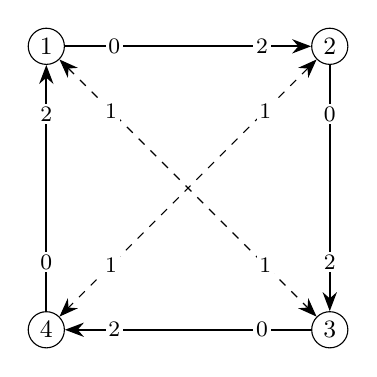
\begin{tikzpicture}[scale=3.6, v/.style={circle,draw,fill=white,inner sep=2pt,font=\small},
  lab/.style={font=\footnotesize,fill=white,inner sep=1pt}, >={Stealth[length=2.4mm]}]
  \node[v] (1) at (0,1) {1};
  \node[v] (2) at (1,1) {2};
  \node[v] (3) at (1,0) {3};
  \node[v] (4) at (0,0) {4};
  \draw[->,thick] (1) -- (2);
  \draw[->,thick] (2) -- (3);
  \draw[->,thick] (3) -- (4);
  \draw[->,thick] (4) -- (1);
  \draw[<->,dashed] (1) -- (3);
  \draw[<->,dashed] (2) -- (4);
  % ranks: label near w on edge wv is r_w(v)
  \path (1) -- (2) node[lab,pos=0.2]{0} node[lab,pos=0.8]{2};
  \path (2) -- (3) node[lab,pos=0.2]{0} node[lab,pos=0.8]{2};
  \path (3) -- (4) node[lab,pos=0.2]{0} node[lab,pos=0.8]{2};
  \path (4) -- (1) node[lab,pos=0.2]{0} node[lab,pos=0.8]{2};
  \path (1) -- (3) node[lab,pos=0.2]{1} node[lab,pos=0.8]{1};
  \path (2) -- (4) node[lab,pos=0.2]{1} node[lab,pos=0.8]{1};
\end{tikzpicture}
\end{center}
In the figure the small number next to vertex $w$ on the edge $wv$ is $r_w(v)$. The arrows show
the digraph $O$ of Step~4: the middle rank is $\half=1$, so the sides of the square, with ranks
$0$ and $2$ at their ends, get one arc each, and the diagonals, with rank $1$ at both ends, get
arcs in both directions (dashed). Every vertex has $2$ out-arcs and $2$ in-arcs, as
Lemma~\ref{lem:O}(d) says.
\begin{itemize}
  \item \emph{Step 6 fails.} $1\to 2\to 3\to 1$ is a directed cycle of $O$ of length $3$: the
    arcs $1\to 2$ and $2\to 3$ are sides, and $3\to 1$ is a diagonal.
  \item \emph{Step 5: it is a ring.} Vertex $1$ prefers $2$ (rank $0$) to $3$ (rank $1$); vertex
    $2$ prefers $3$ (rank $0$) to $1$ (rank $2$); vertex $3$ prefers $1$ (rank $1$) to $2$ (rank
    $2$).
  \item \emph{Step 3: the ring gives a kernel-less triangle in $D$.} At $2$, the edge $12$ (rank
    $2$) points to $23$ (rank $0$); at $3$, the edge $23$ (rank $2$) points to $31$ (rank $1$);
    at $1$, the edge $31$ (rank $1$) points to $12$ (rank $0$). So $12\to 23\to 31\to 12$ is a
    directed triangle in $D$, and $D[\{12,23,31\}]$ has no kernel.
\end{itemize}
\end{example}

\begin{example}[$K_{3,3}$: where certificates exist]\label{ex:k33}
$K_{3,3}$ is $3$-regular and bipartite, so Galvin's theorem gives $3$-certificates. The
brute-force search finds $148$ orientations of $L(K_{3,3})$ with every out-degree at most $2$,
of which exactly $12$ are kernel-perfect. There are exactly $12$ proper edge colourings of
$K_{3,3}$ with colours $0,1,2$ (they are the $3\times 3$ Latin squares), and the search confirms
that the $12$ certificates are exactly the $12$ Galvin orientations, as
Theorem~\ref{thm:rigid} predicts. Steps~1 to~8 all hold for these certificates; Step~8 simply
confirms that every cycle of $K_{3,3}$ is even.
\end{example}

\begin{example}[the diamond: regularity is needed]\label{ex:diamond}
The diamond is $K_4$ minus one edge. It has degrees $3,3,2,2$, so it is not regular; it contains
a triangle, so it is not bipartite; it has $\Delta=3$. The brute-force search finds $72$
orientations of its line graph with every out-degree at most $2$, and exactly $2$ of them are
kernel-perfect. So it has $3$-certificates, and Theorem~\ref{thm:main} fails without regularity.
This agrees with McDonald~\cite[Theorem~3]{mcd}, since the diamond is a $4$-cycle plus one edge,
a bipartite graph plus an edge.
In the proof, Step~2 is what breaks: the slack of Remark~\ref{rem:regular} is $2$ (four edges
join a vertex of degree $3$ to one of degree $2$, each contributing $\tfrac12$), and indeed none
of the $72$ orientations has every out-degree equal to $2$.
\end{example}

%=================================================================================================
\section{Rigidity: every certificate is Galvin's}\label{sec:rigidity}
%=================================================================================================

\begin{definition}[Galvin orientation]\label{def:galvin-orientation}
Let $G$ be a simple bipartite graph with bipartition $(A,B)$, and $c$ a proper edge colouring of
$G$ with colours in $\{0,\dots,k-1\}$. The \emph{Galvin orientation} $D_c$ of $\LG$ is defined
as follows. Let $e,f$ be adjacent edges and $w=w(e,f)$ their common end
(Lemma~\ref{lem:line-graph}(b)); $c(e)\ne c(f)$ because $c$ is proper.
\begin{itemize}
  \item If $w\in A$: $e\to f$ iff $c(e)>c(f)$ (point to the smaller colour).
  \item If $w\in B$: $e\to f$ iff $c(e)<c(f)$ (point to the larger colour).
\end{itemize}
\end{definition}

Swapping the roles of $A$ and $B$ gives the same family of orientations: it equals $D_{c'}$ for
the colouring $c'=k-1-c$. So the convention does not matter.

\begin{lemma}\label{lem:galvin-outdeg}
If $G$ is simple, $k$-regular and bipartite, then in every Galvin orientation $D_c$ each edge has
out-degree exactly $k-1$.
\end{lemma}

\begin{proof}
\begin{steps}
  \item Let $e=ab$ with $a\in A$, $b\in B$. At $a$ there are $k$ edges with $k$ distinct colours
    from $\{0,\dots,k-1\}$, so every colour occurs at $a$ exactly once. The same holds at $b$.
  \item At $a$, $e$ points to the edges of smaller colour: there are $c(e)$ of them.
  \item At $b$, $e$ points to the edges of larger colour: there are $k-1-c(e)$ of them.
  \item Every out-neighbour of $e$ is at $a$ or at $b$, not both
    \why{Lemma~\ref{lem:line-graph}(c)}. So $\dout(e)=c(e)+(k-1-c(e))=k-1$. \qedhere
\end{steps}
\end{proof}

By Galvin's theorem, as proved in~\cite{galvin}, every $D_c$ is kernel-perfect, so by
Lemma~\ref{lem:galvin-outdeg} every $D_c$ is a $k$-certificate. The next theorem is the
converse.

\begin{theorem}[rigidity]\label{thm:rigid}
Let $k\ge 1$ and let $G$ be a simple $k$-regular bipartite graph with bipartition $(A,B)$.
\begin{enumerate}[label=(\alph*)]
  \item For every $k$-certificate $D$ of $G$, the map $c(ab)=r_a(b)$ (for $a\in A$, $b\in B$) is
    a proper edge colouring with colours $0,\dots,k-1$, and $D=D_c$.
  \item This $c$ is the only proper colouring with $D=D_c$.
  \item Consequently, using Galvin's theorem, $c\mapsto D_c$ is a bijection from the proper edge
    colourings of $G$ with colours $0,\dots,k-1$ onto the $k$-certificates of $G$.
\end{enumerate}
\end{theorem}

\begin{proof}
(a) Let $D$ be a $k$-certificate. Standing Hypothesis~\ref{hyp:main} holds, so Steps~1 and~2
apply: ranks exist and $r_a(b)+r_b(a)=k-1$ on every edge.
\begin{steps}
  \item \emph{$c$ is proper at vertices of $A$.} On $\st{a}$, $c$ equals $r_a$, which is
    injective \why{Lemma~\ref{lem:rank}(a)}.
  \item \emph{$c$ is proper at vertices of $B$.} For $ab\in\st{b}$,
    $c(ab)=r_a(b)=k-1-r_b(a)$ \why{Lemma~\ref{lem:tight}}. The map $r_b$ is injective on
    $\st{b}$, and so is $x\mapsto k-1-x$. So $c$ is injective on $\st{b}$.
  \item \emph{$D$ agrees with $D_c$ at vertices of $A$.} For distinct $e,f\in\st{a}$: $e\to f$
    in $D$ iff $r_a(e)>r_a(f)$ \why{Lemma~\ref{lem:rank}(b)} iff $c(e)>c(f)$, which is the rule of
    $D_c$ at $a\in A$.
  \item \emph{$D$ agrees with $D_c$ at vertices of $B$.} For distinct $e,f\in\st{b}$: $e\to f$
    in $D$ iff $r_b(e)>r_b(f)$ iff $k-1-c(e)>k-1-c(f)$ \why{(2)} iff $c(e)<c(f)$, which is the
    rule of $D_c$ at $b\in B$.
  \item Every pair of adjacent edges has exactly one common end
    \why{Lemma~\ref{lem:line-graph}(b)}, which lies in $A$ or in $B$. By (3) and (4), $D$ and
    $D_c$ have the same arc between them. So $D=D_c$.
\end{steps}

(b) \begin{steps}
  \item Suppose $D=D_{c'}$ for a proper colouring $c'$. Let $a\in A$ and $e\in\st{a}$.
  \item In $D_{c'}$, the edge $e$ points, inside $\st{a}$, to exactly the edges of smaller
    colour. The colours on $\st{a}$ are $0,\dots,k-1$, each once (as in
    step (1) of the proof of Lemma~\ref{lem:galvin-outdeg}), so there are $c'(e)$ such edges.
  \item That number is $r_a(e)$ by Definition~\ref{def:rank}. So $c'(e)=r_a(e)=c(e)$.
  \item Every edge has an end in $A$, so $c'=c$.
\end{steps}

(c) By Galvin's theorem and Lemma~\ref{lem:galvin-outdeg}, $c\mapsto D_c$ maps proper colourings
to $k$-certificates. It is injective by (b) (if $D_c=D_{c'}$ then $c=c'$) and onto by (a).
\end{proof}

\begin{remark}
Parts (a) and (b) do not use Galvin's theorem: they say that if a certificate exists, it has
Galvin's form. Only (c), the statement that every $D_c$ really is kernel-perfect, uses it. The
brute-force search confirms the bijection of (c) on $C_4$, $C_6$, $K_{3,3}$ and the cube $Q_3$,
with $2$, $2$, $12$ and $24$ certificates and as many colourings.
\end{remark}

%=================================================================================================
\section{Orientations with arcs in both directions}\label{sec:twoway}
%=================================================================================================

Some authors, for example McDonald and Puleo~\cite{mp}, apply the kernel lemma to digraphs in
which adjacent vertices may be joined by arcs in both directions. The kernel lemma holds in that
setting too: the proof in~\cite[Chapter~33]{book} never uses that two vertices are joined by at
most one arc. Theorem~\ref{thm:main} extends to this setting.

\begin{proposition}\label{prop:twoway}
Let $k\ge 1$ and let $G$ be a simple $k$-regular graph. Let $D$ be a digraph with vertex set $E$
such that
\begin{enumerate}[label=(\roman*)]
  \item every arc of $D$ joins two edges that are adjacent in $\LG$;
  \item every two edges adjacent in $\LG$ are joined by at least one arc (possibly by both);
  \item $D$ is kernel-perfect;
  \item $\dout_D(e)\le k-1$ for every $e$.
\end{enumerate}
Then no two edges are joined by arcs in both directions. So $D$ is a $k$-certificate, and $G$ is
bipartite.
\end{proposition}

\begin{proof}
\begin{steps}
  \item Let $p$ be the number of adjacent pairs joined by both arcs. By (i) and (ii), the number
    of arcs of $D$ is (number of edges of $\LG$) $+\,p$.
  \item By Lemma~\ref{lem:sum-outdeg} and (iv), the number of arcs is
    $\sum_e\dout_D(e)\le|E|(k-1)$.
  \item The number of edges of $\LG$ is $|E|(k-1)$ \why{Lemma~\ref{lem:line-graph}(d)}.
  \item So $|E|(k-1)+p\le|E|(k-1)$, hence $p=0$.
  \item Then $D$ is an orientation of $\LG$ satisfying (C1) and (C2), and
    Theorem~\ref{thm:main} applies. \qedhere
\end{steps}
\end{proof}

%=================================================================================================
\section{Impact and consequences}\label{sec:impact}
%=================================================================================================

This section explains what the result implies and what it leads to. Statements about other
papers are cited, not proved.

\subsection{What it adds to Galvin's theorem}

Galvin's theorem says: bipartite $\Rightarrow$ the kernel method with lists of size $\Delta$
works. Theorem~\ref{thm:main} says: for simple regular graphs, the method works $\Rightarrow$
bipartite. Theorem~\ref{thm:rigid} says: when it works, the only certificates are Galvin's own.
Together they describe the kernel method with lists of size $\Delta$ on simple regular graphs
completely:
\begin{itemize}
  \item it succeeds exactly on the bipartite graphs (Corollary~\ref{cor:char});
  \item where it succeeds, the certificates are exactly the Galvin orientations, one for each
    proper $\Delta$-edge colouring (Theorem~\ref{thm:rigid}).
\end{itemize}
So, on simple regular graphs, Galvin's 1995 construction is not one successful use of the
kernel method among possibly many: it is all of it. Section~\ref{sec:not-automatic} explains why
this was not a foregone conclusion.

The size of the contribution should be stated plainly. It is a \emph{barrier} result, about the
limits of a method. It proves the LECC for no new graph, and it has an elementary proof of about
a page.

\subsection{Which cases of the conjecture it affects}

For a simple regular graph $G$ there are three cases.
\begin{enumerate}[label=(\arabic*)]
  \item \emph{$G$ bipartite.} The LECC holds by Galvin's theorem, and the kernel method is the
    proof.
  \item \emph{$G$ of class two.} Then $\chil(G)\ge\chie(G)=\Delta+1$, so the LECC asks for
    $\chil(G)=\Delta+1$, a question about lists of size $\Delta+1$. Theorem~\ref{thm:main} says
    nothing here.
  \item \emph{$G$ non-bipartite and of class one.} The LECC predicts $\chil(G)=\Delta$.
    Theorem~\ref{thm:main} says the kernel method cannot prove this, for any such $G$.
\end{enumerate}
Case (3) is a large part of the conjecture. It contains:
\begin{itemize}
  \item \emph{Complete graphs of even order.} $K_{2n}$ ($n\ge 2$) is $(2n-1)$-regular, of class
    one, and not bipartite. The LECC for $K_{2n}$ is open in general; it is known when $2n-1$ is
    an odd prime (Schauz~\cite{schauz14}) and for further families (Jafari~\cite{jafari}), all by
    algebraic methods. Theorem~\ref{thm:main} explains why no kernel proof has appeared: none
    exists. It contains our earlier result that $L(K_{2n})$ has no $(2n-1)$-certificate
    (\path{list-colouring/12-theorem-even-complete.md}), and strengthens, for complete graphs of even order, McDonald's result~\cite{mcd},
    which excludes only certificates of Galvin's form. ($K_{2n+1}$ is of class two, case (2).)
  \item \emph{Planar regular class-one graphs that are not bipartite}, such as $K_4$, the
    octahedron, the triangular prism and the pentagonal prism $C_5\square K_2$. Ellingham and
    Goddyn~\cite{eg} proved the LECC for every $d$-regular $d$-edge-colourable planar graph, by
    the Alon and Tarsi method~\cite{at}. By Theorem~\ref{thm:main}, the kernel method could not
    have proved it for the non-bipartite ones. The brute-force search confirms this directly for
    $K_4$, the octahedron and both prisms (Section~\ref{sec:computation}).
  \item \emph{Schauz's open small graphs.} Schauz~\cite{schauz17} proved the LECC for most graphs
    on at most $10$ vertices by the Alon and Tarsi method. He left open the regular class-one
    graphs on which the relevant coefficient vanishes: $3$ on $8$ vertices and $51$ on $10$. We
    reproduced this census (\path{lecc-small/RESULTS.md}, R1). Of these, $52$ are covered by no
    known theorem, and none of the $52$ is bipartite, so by Theorem~\ref{thm:main} the kernel
    method fails on every one of them.
  \item \emph{Cubic class-one graphs with a triangle.} Our earlier triangle theorem
    (\path{list-colouring/11-triangle-theorem.md}) says these have no $3$-certificate. It is the special case of
    Theorem~\ref{thm:main} with $k=3$ and an odd cycle of length $3$.
\end{itemize}

\subsection{Both standard methods fail on the same open cases}

The two standard tools for the LECC are the kernel method and the Alon and Tarsi polynomial
method~\cite{at}. For a $k$-regular graph $G$, the Alon and Tarsi method with lists of size $k$
also has very little room, for a counting reason of the same kind as Step~2. The graph
polynomial of $\LG$ is a product of one linear factor per edge of $\LG$, so it is homogeneous of
degree $|E|(k-1)$ (Lemma~\ref{lem:line-graph}(d)) in $|E|$ variables. A monomial usable with lists
of size $k$ has every exponent at most $k-1$, and its total degree is $|E|(k-1)$, so every
exponent must equal $k-1$. Only one monomial is usable, and on Schauz's open graphs its
coefficient is zero. So:
\begin{itemize}
  \item on the $52$ open graphs, \emph{both} standard methods provably fail: Alon and Tarsi by
    the census, the kernel method by Theorem~\ref{thm:main}. This explains why they are open,
    and it is why a third method was needed. A SAT-based search over list assignments
    (\path{lecc-small/RESULTS.md}; the general approach is that
    of~\cite{kpss}) has since settled $6$ of them;
  \item the two methods are \emph{incomparable} on regular graphs. Alon and Tarsi proves
    $\chil(K_4)=3$ (a case of the Ellingham and Goddyn theorem), where the kernel method cannot. In the
    other direction, two of Schauz's zero-sum graphs on $10$ vertices are bipartite, one of them
    $K_{5,5}$ (\path{lecc-small/RESULTS.md}, R2): there the uniform coefficient is zero, so
    Alon and Tarsi with lists of size $k$ fails, while Galvin's kernel method works.
\end{itemize}
Any attack on case (3) must therefore start from the Alon and Tarsi side in a stronger form, or
from a new idea.

\subsection{The limits of the statement}

\begin{itemize}
  \item \emph{Not a lower bound on $\chil$.} It does not say $\chil(G)>\Delta$; $K_4$ shows that
    would be false (Section~\ref{sec:not-say}).
  \item \emph{Regular graphs only.} The diamond shows this is necessary
    (Example~\ref{ex:diamond}); regularity is used exactly once, in Step~2
    (Remark~\ref{rem:regular}).
  \item \emph{Lists of size $\Delta$ only.} With lists of size $\Delta+1$ the kernel method
    succeeds on non-bipartite regular graphs: the brute-force search finds $6$ kernel-perfect
    orientations of $L(K_4)$ and $648$ of the line graph of the triangular prism with every
    out-degree at most $3$ (Section~\ref{sec:computation}). McDonald~\cite[Theorem~4]{mcd}
    shows the Petersen graph also has one. For class-one graphs this gives only $\chil\le\Delta+1$, not the
    conjectured value.
  \item \emph{Simple graphs only.} The multigraph case is open (Remark~\ref{rem:simple}).
  \item \emph{The kernel lemma only.} It says nothing about other methods that use orientations,
    such as Alon and Tarsi.
\end{itemize}

\subsection{Questions it leads to}

\begin{question}[multigraphs]
Is Theorem~\ref{thm:main} true for regular multigraphs? Galvin's theorem holds for bipartite
multigraphs, so the natural statement is again a characterisation. The proof breaks at
Lemma~\ref{lem:rank}(c), where two parallel edges share two stars.
\end{question}

\begin{question}[the least budget]
For a non-bipartite regular class-one graph $G$, what is the least $t$ such that $G$ has a
$t$-certificate? Theorem~\ref{thm:main} says $t\ge\Delta+1$, and for $K_4$ and the triangular
prism the search shows $t=\Delta+1$. Is $t=\Delta+1$ for every such graph? This is the
regular-graph version of McDonald's question~\cite{mcd} for Galvin orientations, asked for all
orientations.
\end{question}

\begin{question}[near-regular graphs]
Remark~\ref{rem:regular} measures the distance from regularity by the slack
$\sum_{uv}\bigl(\Delta-\tfrac{d(u)+d(v)}{2}\bigr)$. When the slack is small, almost every
out-degree is forced to be $\Delta-1$. Is there a quantitative version of
Theorem~\ref{thm:main}, for example one in which an odd cycle far from the vertices of degree
less than $\Delta$ forbids a $\Delta$-certificate?
\end{question}

\begin{question}[a method for case (3)]
Both standard methods fail on Schauz's $52$ open graphs. Is there a general method that works on
non-bipartite regular class-one graphs, or a structural reason that makes them hard?
\end{question}

%=================================================================================================
\section{Computational confirmation}\label{sec:computation}
%=================================================================================================

The proof does not depend on any computation. The computations below check it independently.

\paragraph{Brute force, using no lemma.} The script
\path{lecc-small/reverse_galvin_checks.py} (pure Python, about $30$ seconds) does the
following for each graph $G$ in Table~\ref{tab:brute}, with $k=\Delta(G)$:
\begin{enumerate}[label=(\arabic*)]
  \item it lists every orientation of $\LG$ with every out-degree at most $k-1$;
  \item it tests each one for kernel-perfectness directly from Definition~\ref{def:kernel-intro},
    by searching every induced subdigraph for a kernel;
  \item it counts the proper edge colourings with colours $0,\dots,k-1$;
  \item for the regular bipartite graphs, it checks that the set of certificates equals the set
    of Galvin orientations $D_c$ and that $c\mapsto D_c$ is injective (Theorem~\ref{thm:rigid}).
\end{enumerate}
It uses none of the lemmas of this document. Its output is
\path{lecc-small/data/reverse_galvin_checks.out}.

\begin{table}[ht]
\centering
\small
\begin{tabular}{@{}lccccrrrc@{}}
\toprule
$G$ & $k$ & regular & bipartite & class & orient. & all $\dout=k-1$ & certificates & colourings \\
\midrule
$C_4$ & 2 & yes & yes & 1 & 2 & 2 & 2 & 2 \\
$C_5$ & 2 & yes & no & 2 & 2 & 2 & 0 & 0 \\
$C_6$ & 2 & yes & yes & 1 & 2 & 2 & 2 & 2 \\
$K_4$ & 3 & yes & no & 1 & 38 & 38 & 0 & 6 \\
$K_{3,3}$ & 3 & yes & yes & 1 & 148 & 148 & 12 & 12 \\
prism $K_3\square K_2$ & 3 & yes & no & 1 & 154 & 154 & 0 & 6 \\
cube $Q_3$ & 3 & yes & yes & 1 & 600 & 600 & 24 & 24 \\
$C_5\square K_2$ & 3 & yes & no & 1 & 2466 & 2466 & 0 & 30 \\
Petersen & 3 & yes & no & 2 & 2336 & 2336 & 0 & 0 \\
$K_5$ & 4 & yes & no & 2 & 47504 & 47504 & 0 & 0 \\
octahedron & 4 & yes & no & 1 & 325744 & 325744 & 0 & 48 \\
diamond & 3 & no & no & 1 & 72 & 0 & 2 & 6 \\
\bottomrule
\end{tabular}
\caption{Brute force. ``orient.'' counts orientations of $\LG$ with every out-degree at most
$k-1$; ``all $\dout=k-1$'' counts those in which every out-degree equals $k-1$;
``certificates'' counts the kernel-perfect ones; ``colourings'' counts proper edge colourings
with colours $0,\dots,k-1$ (so it is $0$ exactly for class two). The class column follows from
the colourings column.}
\label{tab:brute}
\end{table}

What the table shows:
\begin{itemize}
  \item \emph{Theorem~\ref{thm:main}:} every regular non-bipartite graph has $0$ certificates,
    including the class-one graphs $K_4$, both prisms and the octahedron.
  \item \emph{Corollary~\ref{cor:char} and Theorem~\ref{thm:rigid}:} every regular bipartite
    graph has certificates, exactly as many as colourings, and they are the Galvin orientations
    (the script reports ``ok'' for each).
  \item \emph{Step~2:} for every regular graph the two orientation counts agree: every
    orientation with out-degrees at most $k-1$ has all out-degrees exactly $k-1$. For the
    non-regular diamond they do not.
  \item \emph{Regularity is needed:} the diamond has $2$ certificates.
\end{itemize}
The same script also counts kernel-perfect orientations with every out-degree at most $k$
(lists of size $k+1$): $6$ for $K_4$ (out of $2608$ orientations) and $648$ for the triangular
prism (out of $132864$).

\paragraph{Larger census, using the odd-ring reduction.} The SAT search
\path{lecc-small/kernel_sat.py} decides whether a $k$-certificate exists for every connected
regular graph on $6$ and $8$ vertices (every degree from $3$), on $10$ vertices (degrees $3$ to
$7$), for cubic graphs on $12$ vertices, triangle-free cubic graphs on $14$ vertices and
$4$-regular graphs on $12$ vertices: $1923$ graphs. A certificate exists exactly for the $29$
bipartite ones (\path{lecc-small/data/kernel_all_small.csv},
\path{lecc-small/data/kernel_N12_k4.csv}). This search encodes Steps~1 and~2 and the full
odd-cycle characterisation of Borodin, Kostochka and Woodall~\cite{bkw}, so it is not
independent of the ideas of the proof, but it does not use Steps~4 to~8.

%=================================================================================================
\section{Novelty and status}\label{sec:novelty}
%=================================================================================================

We have not found Theorem~\ref{thm:main} or Theorem~\ref{thm:rigid} in the literature. The
search is recorded in \path{lecc-small/05-novelty-check.md}. We checked:
\begin{itemize}
  \item Borodin, Kostochka and Woodall~\cite{bkw}: they characterise which orientations of a
    line graph are kernel-perfect, not which graphs admit one within the budget $\Delta$;
  \item McDonald~\cite{mcd}: negative results only for Galvin's special form of orientation, for
    $K_n$ and for one non-regular graph;
  \item McDonald and Puleo~\cite{mp}: consistent with Proposition~\ref{prop:twoway}; no
    non-bipartite regular graph of degree at least $3$ lies in their class;
  \item the papers citing~\cite{bkw}, and recent work on the LECC for complete
    graphs~\cite{jafari}.
\end{itemize}
Two sources could not be checked: the 2016 Auburn M.Sc.\ thesis of A.~Blumenthal, \emph{On
Galvin's Theorem and Stable Matchings}~\cite{blumenthal}, and Woodall's 2001
survey~\cite{woodall}. Since the proof is short and elementary, the result may be known to
specialists without being published. It should be described as ``not found in the
literature'', not as new, until those two sources are checked.

%=================================================================================================
\begin{thebibliography}{99}
%=================================================================================================

\bibitem{book} M.~Aigner and G.~M.~Ziegler, \emph{Proofs from THE BOOK}, fourth edition,
  Springer, 2010. Chapter 33, ``The Dinitz problem''.

\bibitem{at} N.~Alon and M.~Tarsi, Colorings and orientations of graphs, \emph{Combinatorica}
  12 (1992), pages 125 to 134.

\bibitem{blumenthal} A.~Blumenthal, \emph{On Galvin's Theorem and Stable Matchings}, M.Sc.\
  thesis, Auburn University, 2016.

\bibitem{bkw} O.~V.~Borodin, A.~V.~Kostochka and D.~R.~Woodall, On kernel-perfect orientations
  of line graphs, \emph{Discrete Mathematics} 191 (1998), pages 45 to 49.

\bibitem{eg} M.~N.~Ellingham and L.~Goddyn, List edge colourings of some 1-factorable
  multigraphs, \emph{Combinatorica} 16 (1996), pages 343 to 352.

\bibitem{galvin} F.~Galvin, The list chromatic index of a bipartite multigraph, \emph{Journal of
  Combinatorial Theory, Series B} 63 (1995), pages 153 to 158.

\bibitem{jafari} A.~Jafari, The list edge-coloring conjecture for new infinite families,
  arXiv:2608.22895 (2026).

\bibitem{kpss} M.~Kirchweger, T.~Peitl, D.~Seka and S.~Szeider, Graph choosability via SAT:
  beyond the Nullstellensatz, \emph{Proceedings of AAAI} (2026).

\bibitem{konig} D.~K\H{o}nig, \"Uber Graphen und ihre Anwendung auf Determinantentheorie und
  Mengenlehre, \emph{Mathematische Annalen} 77 (1916), pages 453 to 465.

\bibitem{mcd} J.~McDonald, On Galvin orientations of line graphs and list-edge-colouring,
  arXiv:1508.01820 (2015).

\bibitem{mp} J.~McDonald and G.~J.~Puleo, The list chromatic index of simple graphs whose odd
  cycles intersect in at most one edge, \emph{Discrete Mathematics} (2017), arXiv:1507.05933.

\bibitem{schauz14} U.~Schauz, Proof of the list edge coloring conjecture for complete graphs of
  prime degree, \emph{Electronic Journal of Combinatorics} 21(3) (2014), paper P3.43.

\bibitem{schauz17} U.~Schauz, Orientations of 1-factorizations and the list chromatic index of
  small graphs, arXiv:1705.00484 (2017); \emph{Journal of Discrete Algorithms} 52 and 53 (2018),
  pages 182 to 191.

\bibitem{vizing} V.~G.~Vizing, On an estimate of the chromatic class of a $p$-graph,
  \emph{Diskretny\u{\i} Analiz} 3 (1964), pages 25 to 30.

\bibitem{woodall} D.~R.~Woodall, List colourings of graphs, in \emph{Surveys in Combinatorics
  2001}, London Mathematical Society Lecture Note Series 288, Cambridge University Press, 2001.

\end{thebibliography}

\end{document}
